% GNUPLOT: LaTeX picture with Postscript
\begingroup
  \makeatletter
  \providecommand\color[2][]{%
    \GenericError{(gnuplot) \space\space\space\@spaces}{%
      Package color not loaded in conjunction with
      terminal option `colourtext'%
    }{See the gnuplot documentation for explanation.%
    }{Either use 'blacktext' in gnuplot or load the package
      color.sty in LaTeX.}%
    \renewcommand\color[2][]{}%
  }%
  \providecommand\includegraphics[2][]{%
    \GenericError{(gnuplot) \space\space\space\@spaces}{%
      Package graphicx or graphics not loaded%
    }{See the gnuplot documentation for explanation.%
    }{The gnuplot epslatex terminal needs graphicx.sty or graphics.sty.}%
    \renewcommand\includegraphics[2][]{}%
  }%
  \providecommand\rotatebox[2]{#2}%
  \@ifundefined{ifGPcolor}{%
    \newif\ifGPcolor
    \GPcolorfalse
  }{}%
  \@ifundefined{ifGPblacktext}{%
    \newif\ifGPblacktext
    \GPblacktexttrue
  }{}%
  % define a \g@addto@macro without @ in the name:
  \let\gplgaddtomacro\g@addto@macro
  % define empty templates for all commands taking text:
  \gdef\gplbacktext{}%
  \gdef\gplfronttext{}%
  \makeatother
  \ifGPblacktext
    % no textcolor at all
    \def\colorrgb#1{}%
    \def\colorgray#1{}%
  \else
    % gray or color?
    \ifGPcolor
      \def\colorrgb#1{\color[rgb]{#1}}%
      \def\colorgray#1{\color[gray]{#1}}%
      \expandafter\def\csname LTw\endcsname{\color{white}}%
      \expandafter\def\csname LTb\endcsname{\color{black}}%
      \expandafter\def\csname LTa\endcsname{\color{black}}%
      \expandafter\def\csname LT0\endcsname{\color[rgb]{1,0,0}}%
      \expandafter\def\csname LT1\endcsname{\color[rgb]{0,1,0}}%
      \expandafter\def\csname LT2\endcsname{\color[rgb]{0,0,1}}%
      \expandafter\def\csname LT3\endcsname{\color[rgb]{1,0,1}}%
      \expandafter\def\csname LT4\endcsname{\color[rgb]{0,1,1}}%
      \expandafter\def\csname LT5\endcsname{\color[rgb]{1,1,0}}%
      \expandafter\def\csname LT6\endcsname{\color[rgb]{0,0,0}}%
      \expandafter\def\csname LT7\endcsname{\color[rgb]{1,0.3,0}}%
      \expandafter\def\csname LT8\endcsname{\color[rgb]{0.5,0.5,0.5}}%
    \else
      % gray
      \def\colorrgb#1{\color{black}}%
      \def\colorgray#1{\color[gray]{#1}}%
      \expandafter\def\csname LTw\endcsname{\color{white}}%
      \expandafter\def\csname LTb\endcsname{\color{black}}%
      \expandafter\def\csname LTa\endcsname{\color{black}}%
      \expandafter\def\csname LT0\endcsname{\color{black}}%
      \expandafter\def\csname LT1\endcsname{\color{black}}%
      \expandafter\def\csname LT2\endcsname{\color{black}}%
      \expandafter\def\csname LT3\endcsname{\color{black}}%
      \expandafter\def\csname LT4\endcsname{\color{black}}%
      \expandafter\def\csname LT5\endcsname{\color{black}}%
      \expandafter\def\csname LT6\endcsname{\color{black}}%
      \expandafter\def\csname LT7\endcsname{\color{black}}%
      \expandafter\def\csname LT8\endcsname{\color{black}}%
    \fi
  \fi
    \setlength{\unitlength}{0.0500bp}%
    \ifx\gptboxheight\undefined%
      \newlength{\gptboxheight}%
      \newlength{\gptboxwidth}%
      \newsavebox{\gptboxtext}%
    \fi%
    \setlength{\fboxrule}{0.5pt}%
    \setlength{\fboxsep}{1pt}%
    \definecolor{tbcol}{rgb}{1,1,1}%
\begin{picture}(7200.00,7200.00)%
    \gplgaddtomacro\gplbacktext{%
      \csname LTb\endcsname%%
      \put(814,216){\makebox(0,0)[r]{\strut{}$-25$}}%
      \csname LTb\endcsname%%
      \put(814,824){\makebox(0,0)[r]{\strut{}$-20$}}%
      \csname LTb\endcsname%%
      \put(814,1431){\makebox(0,0)[r]{\strut{}$-15$}}%
      \csname LTb\endcsname%%
      \put(814,2039){\makebox(0,0)[r]{\strut{}$-10$}}%
      \csname LTb\endcsname%%
      \put(814,2647){\makebox(0,0)[r]{\strut{}$-5$}}%
      \csname LTb\endcsname%%
      \put(814,3255){\makebox(0,0)[r]{\strut{}$0$}}%
      \csname LTb\endcsname%%
      \put(814,3862){\makebox(0,0)[r]{\strut{}$5$}}%
      \csname LTb\endcsname%%
      \put(814,4470){\makebox(0,0)[r]{\strut{}$10$}}%
      \csname LTb\endcsname%%
      \put(814,5078){\makebox(0,0)[r]{\strut{}$15$}}%
      \csname LTb\endcsname%%
      \put(814,5685){\makebox(0,0)[r]{\strut{}$20$}}%
      \csname LTb\endcsname%%
      \put(814,6293){\makebox(0,0)[r]{\strut{}$25$}}%
      \csname LTb\endcsname%%
      \put(946,-4){\makebox(0,0){\strut{}$-20$}}%
      \csname LTb\endcsname%%
      \put(1554,-4){\makebox(0,0){\strut{}$-15$}}%
      \csname LTb\endcsname%%
      \put(2162,-4){\makebox(0,0){\strut{}$-10$}}%
      \csname LTb\endcsname%%
      \put(2769,-4){\makebox(0,0){\strut{}$-5$}}%
      \csname LTb\endcsname%%
      \put(3377,-4){\makebox(0,0){\strut{}$0$}}%
      \csname LTb\endcsname%%
      \put(3985,-4){\makebox(0,0){\strut{}$5$}}%
      \csname LTb\endcsname%%
      \put(4593,-4){\makebox(0,0){\strut{}$10$}}%
      \csname LTb\endcsname%%
      \put(5200,-4){\makebox(0,0){\strut{}$15$}}%
      \csname LTb\endcsname%%
      \put(5808,-4){\makebox(0,0){\strut{}$20$}}%
    }%
    \gplgaddtomacro\gplfronttext{%
      \csname LTb\endcsname%%
      \put(209,3254){\rotatebox{-270.00}{\makebox(0,0){\strut{}y (cm)}}}%
      \put(3377,-334){\makebox(0,0){\strut{}x (cm)}}%
      \put(6305,216){\makebox(0,0)[l]{\strut{}1.5 V}}%
      \put(6305,1084){\makebox(0,0)[l]{\strut{}2.0 V}}%
      \put(6305,1952){\makebox(0,0)[l]{\strut{}2.3 V}}%
      \put(6305,2820){\makebox(0,0)[l]{\strut{}2.5 V}}%
      \put(6305,3688){\makebox(0,0)[l]{\strut{}2.7 V}}%
      \put(6305,4556){\makebox(0,0)[l]{\strut{}3.0 V}}%
      \put(6305,5424){\makebox(0,0)[l]{\strut{}3.3 V}}%
      \put(6305,6293){\makebox(0,0)[l]{\strut{}4.0 V}}%
    }%
    \gplbacktext
    \put(0,0){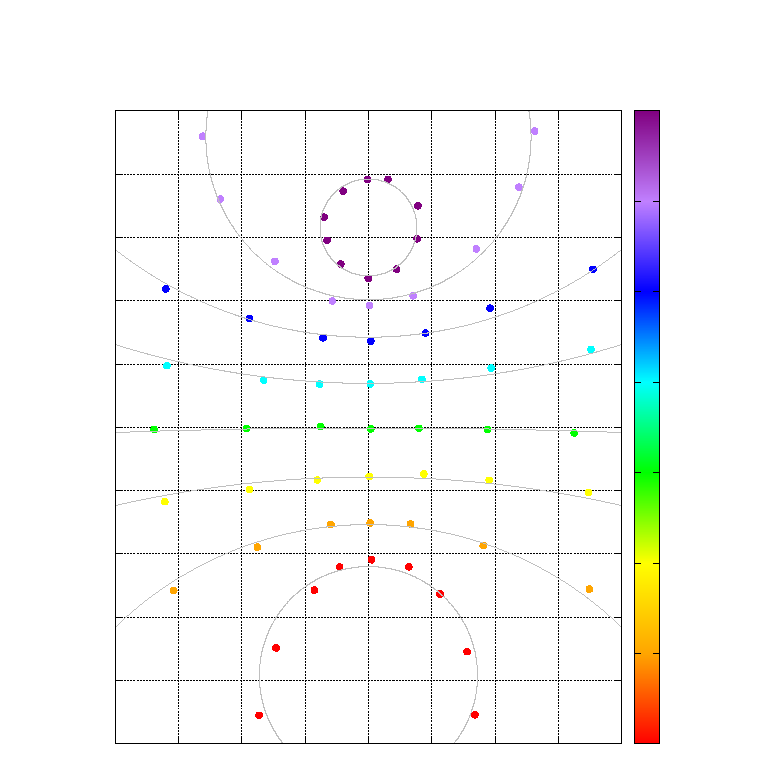
\includegraphics[width={360.00bp},height={360.00bp}]{plochy}}%
    \gplfronttext
  \end{picture}%
\endgroup
